\documentclass[twoside]{book}

% Packages required by doxygen
\usepackage{fixltx2e}
\usepackage{calc}
\usepackage{doxygen}
\usepackage[export]{adjustbox} % also loads graphicx
\usepackage{graphicx}
\usepackage[utf8]{inputenc}
\usepackage{makeidx}
\usepackage{multicol}
\usepackage{multirow}
\PassOptionsToPackage{warn}{textcomp}
\usepackage{textcomp}
\usepackage[nointegrals]{wasysym}
\usepackage[table]{xcolor}

% Font selection
\usepackage[T1]{fontenc}
\usepackage[scaled=.90]{helvet}
\usepackage{courier}
\usepackage{amssymb}
\usepackage{sectsty}
\renewcommand{\familydefault}{\sfdefault}
\allsectionsfont{%
  \fontseries{bc}\selectfont%
  \color{darkgray}%
}
\renewcommand{\DoxyLabelFont}{%
  \fontseries{bc}\selectfont%
  \color{darkgray}%
}
\newcommand{\+}{\discretionary{\mbox{\scriptsize$\hookleftarrow$}}{}{}}

% Page & text layout
\usepackage{geometry}
\geometry{%
  a4paper,%
  top=2.5cm,%
  bottom=2.5cm,%
  left=2.5cm,%
  right=2.5cm%
}
\tolerance=750
\hfuzz=15pt
\hbadness=750
\setlength{\emergencystretch}{15pt}
\setlength{\parindent}{0cm}
\setlength{\parskip}{3ex plus 2ex minus 2ex}
\makeatletter
\renewcommand{\paragraph}{%
  \@startsection{paragraph}{4}{0ex}{-1.0ex}{1.0ex}{%
    \normalfont\normalsize\bfseries\SS@parafont%
  }%
}
\renewcommand{\subparagraph}{%
  \@startsection{subparagraph}{5}{0ex}{-1.0ex}{1.0ex}{%
    \normalfont\normalsize\bfseries\SS@subparafont%
  }%
}
\makeatother

% Headers & footers
\usepackage{fancyhdr}
\pagestyle{fancyplain}
\fancyhead[LE]{\fancyplain{}{\bfseries\thepage}}
\fancyhead[CE]{\fancyplain{}{}}
\fancyhead[RE]{\fancyplain{}{\bfseries\leftmark}}
\fancyhead[LO]{\fancyplain{}{\bfseries\rightmark}}
\fancyhead[CO]{\fancyplain{}{}}
\fancyhead[RO]{\fancyplain{}{\bfseries\thepage}}
\fancyfoot[LE]{\fancyplain{}{}}
\fancyfoot[CE]{\fancyplain{}{}}
\fancyfoot[RE]{\fancyplain{}{\bfseries\scriptsize Generated by Doxygen }}
\fancyfoot[LO]{\fancyplain{}{\bfseries\scriptsize Generated by Doxygen }}
\fancyfoot[CO]{\fancyplain{}{}}
\fancyfoot[RO]{\fancyplain{}{}}
\renewcommand{\footrulewidth}{0.4pt}
\renewcommand{\chaptermark}[1]{%
  \markboth{#1}{}%
}
\renewcommand{\sectionmark}[1]{%
  \markright{\thesection\ #1}%
}

% Indices & bibliography
\usepackage{natbib}
\usepackage[titles]{tocloft}
\setcounter{tocdepth}{3}
\setcounter{secnumdepth}{5}
\makeindex

% Hyperlinks (required, but should be loaded last)
\usepackage{ifpdf}
\ifpdf
  \usepackage[pdftex,pagebackref=true]{hyperref}
\else
  \usepackage[ps2pdf,pagebackref=true]{hyperref}
\fi
\hypersetup{%
  colorlinks=true,%
  linkcolor=blue,%
  citecolor=blue,%
  unicode%
}

% Custom commands
\newcommand{\clearemptydoublepage}{%
  \newpage{\pagestyle{empty}\cleardoublepage}%
}

\usepackage{caption}
\captionsetup{labelsep=space,justification=centering,font={bf},singlelinecheck=off,skip=4pt,position=top}

%===== C O N T E N T S =====

\begin{document}

% Titlepage & ToC
\hypersetup{pageanchor=false,
             bookmarksnumbered=true,
             pdfencoding=unicode
            }
\pagenumbering{roman}
\begin{titlepage}
\vspace*{7cm}
\begin{center}%
{\Large assignment1 }\\
\vspace*{1cm}
{\large Generated by Doxygen 1.8.11}\\
\end{center}
\end{titlepage}
\clearemptydoublepage
\tableofcontents
\clearemptydoublepage
\pagenumbering{arabic}
\hypersetup{pageanchor=true}

%--- Begin generated contents ---
\chapter{Research Track I -\/ first assignment}
\label{md_README}
\hypertarget{md_README}{}
The assignment requires controlling a holonomic robot in a 2d space with a simple 2d simulator, Stage. The simulator can be launched by executing the command\+:


\begin{DoxyCode}
1 rosrun stage\_ros stageros $(rospack find assignment1)/world/exercise.world
\end{DoxyCode}


\subsubsection*{The following behaviour should be achieved}


\begin{DoxyItemize}
\item 1. The robot asks for a random target, with both coordinates in the interval (-\/6.\+0, 6.\+0).
\item 2. The robot reaches the target.
\item 3. Go to step 1.
\end{DoxyItemize}

\subsubsection*{Consider the following requirements}


\begin{DoxyItemize}
\item A new R\+OS packages should be created.
\item Two processes (R\+OS nodes) should be developed.
\item You may use cpp or python for writing your code.
\item The first process will be in charge of\+:
\begin{DoxyItemize}
\item calling a service for receiving a random target;
\item making the robot reach the target.
\end{DoxyItemize}
\item The second process will act as a Service Server, by replying to the client with a random target, having x and y in the interval (-\/6.\+0, 6.\+0).
\item A target is considered reached when the distance between the robot and the target is below 0.\+1.
\end{DoxyItemize}

\subsubsection*{Some hints}


\begin{DoxyItemize}
\item The first node should implement a R\+OS publisher (cmd\+\_\+vel, for setting the robot speed), a R\+OS subscriber (odom, for knowing the actual robot position) and a R\+OS client (for receiving the random target)
\item The second node should implement a R\+OS server (for setting the random target)
\item The position of the robot is given in the topic {\bfseries odom}, by using a {\bfseries nav\+\_\+msgs/\+Odometry} (Odometry message defined in the package nav\+\_\+msgs) message. This means that the x and y position of the robot may be retrieved by reading the pose.\+pose.\+position.\+x and pose.\+pose.\+position.\+y fields of the message received by the callback associated with the subscriber.
\item For the robot control, at first, check if the position has been reached. If yes, you should call the service to retrieve the new target position. If not, you should set {\bfseries cmd\+\_\+vel} (a {\bfseries geometry\+\_\+msgs/\+Twist} message) depending on the difference between the target (xt) and the robot position (x) (e.\+g., vel\+\_\+x = k$\ast$ (xt -\/ x))
\end{DoxyItemize}

\subsubsection*{How to submit the assignment\+:}


\begin{DoxyItemize}
\item The link of a github repository containing the developed R\+OS package should be given;
\item The repo should have a \hyperlink{_r_e_a_d_m_e_8md}{R\+E\+A\+D\+M\+E.\+md} file with\+:
\begin{DoxyItemize}
\item Description of the content of the package (nodes, custom messages or services (if any)).
\item Computational graph of the system (how do nodes communicate? You may use rqt\+\_\+graph).
\item Instructions about how to run the code.
\end{DoxyItemize}
\item Functions and source files should be documented (optional\+: you can create a docs folder with Doxy\+Gen documentation).
\end{DoxyItemize}

\subsubsection*{Deadline}

A soft deadline is set to the 25th November and the next Research Track class will be on November 26th. This means that\+:
\begin{DoxyItemize}
\item You can actually submit your assignment at any time, however 10 days before the oral discussion.
\item I strongly advise you to start working on the assignment in the next weeks. Indeed, in the last 9 hours of the course, we are going to work on more complex robotic simulations, which require a good knowledge of R\+OS. Doing the assignment will be a good way to understand what it is still unclear and catch up with the course.
\item In the next two weeks, you can contact me even outside class hours for clarifications about the assignment and the course subjects in general. 
\end{DoxyItemize}
\chapter{Namespace Index}
\section{Namespace List}
Here is a list of all namespaces with brief descriptions\+:\begin{DoxyCompactList}
\item\contentsline{section}{\hyperlink{namespacerobot__controller}{robot\+\_\+controller} }{\pageref{namespacerobot__controller}}{}
\item\contentsline{section}{\hyperlink{namespacetarget__server}{target\+\_\+server} }{\pageref{namespacetarget__server}}{}
\end{DoxyCompactList}

\chapter{File Index}
\section{File List}
Here is a list of all files with brief descriptions\+:\begin{DoxyCompactList}
\item\contentsline{section}{scripts/\hyperlink{robot__controller_8py}{robot\+\_\+controller.\+py} }{\pageref{robot__controller_8py}}{}
\item\contentsline{section}{scripts/\hyperlink{target__server_8py}{target\+\_\+server.\+py} }{\pageref{target__server_8py}}{}
\item\contentsline{section}{src/\hyperlink{robot__controller_8cpp}{robot\+\_\+controller.\+cpp} }{\pageref{robot__controller_8cpp}}{}
\item\contentsline{section}{src/\hyperlink{target__server_8cpp}{target\+\_\+server.\+cpp} }{\pageref{target__server_8cpp}}{}
\end{DoxyCompactList}

\chapter{Namespace Documentation}
\hypertarget{namespacerobot__controller}{}\section{robot\+\_\+controller Namespace Reference}
\label{namespacerobot__controller}\index{robot\+\_\+controller@{robot\+\_\+controller}}
\subsection*{Functions}
\begin{DoxyCompactItemize}
\item 
def \hyperlink{namespacerobot__controller_ad432a00343321fec384e1e79b142ac5a}{position\+Callback} (pos)
\begin{DoxyCompactList}\small\item\em callback function after subscribing for robot position \end{DoxyCompactList}\item 
def \hyperlink{namespacerobot__controller_accbf10a6a15201c2588764d5481947e7}{main} ()
\begin{DoxyCompactList}\small\item\em main function to call target service and subsrcibe for robot position \end{DoxyCompactList}\end{DoxyCompactItemize}
\subsection*{Variables}
\begin{DoxyCompactItemize}
\item 
\hyperlink{namespacerobot__controller_ac9cb673d888175b8d312b09650d380c9}{pub\+\_\+vel} = rospy.\+Publisher(\textquotesingle{}/cmd\+\_\+vel\textquotesingle{}, Twist, queue\+\_\+size=10)
\begin{DoxyCompactList}\small\item\em publisher to publish robot velocity \end{DoxyCompactList}\item 
\hyperlink{namespacerobot__controller_a091c74e8004fd80216a8b14f8354153d}{client} = rospy.\+Service\+Proxy(\textquotesingle{}/\hyperlink{namespacerobot__controller_af6e678d9713033f52d7fb793cc429b98}{target}\textquotesingle{},Target)
\begin{DoxyCompactList}\small\item\em client to request a target \end{DoxyCompactList}\item 
float \hyperlink{namespacerobot__controller_a0fff075c754060ec1d6a45e42c22bc4a}{distance} = 1000.\+0
\begin{DoxyCompactList}\small\item\em distance between robot and target \end{DoxyCompactList}\item 
\hyperlink{namespacerobot__controller_af6e678d9713033f52d7fb793cc429b98}{target} = Odometry()
\begin{DoxyCompactList}\small\item\em target to be achieved \end{DoxyCompactList}\end{DoxyCompactItemize}


\subsection{Function Documentation}
\index{robot\+\_\+controller@{robot\+\_\+controller}!main@{main}}
\index{main@{main}!robot\+\_\+controller@{robot\+\_\+controller}}
\subsubsection[{\texorpdfstring{main()}{main()}}]{\setlength{\rightskip}{0pt plus 5cm}def robot\+\_\+controller.\+main (
\begin{DoxyParamCaption}
{}
\end{DoxyParamCaption}
)}\hypertarget{namespacerobot__controller_accbf10a6a15201c2588764d5481947e7}{}\label{namespacerobot__controller_accbf10a6a15201c2588764d5481947e7}


main function to call target service and subsrcibe for robot position 

\index{robot\+\_\+controller@{robot\+\_\+controller}!position\+Callback@{position\+Callback}}
\index{position\+Callback@{position\+Callback}!robot\+\_\+controller@{robot\+\_\+controller}}
\subsubsection[{\texorpdfstring{position\+Callback(pos)}{positionCallback(pos)}}]{\setlength{\rightskip}{0pt plus 5cm}def robot\+\_\+controller.\+position\+Callback (
\begin{DoxyParamCaption}
\item[{}]{pos}
\end{DoxyParamCaption}
)}\hypertarget{namespacerobot__controller_ad432a00343321fec384e1e79b142ac5a}{}\label{namespacerobot__controller_ad432a00343321fec384e1e79b142ac5a}


callback function after subscribing for robot position 


\begin{DoxyParams}{Parameters}
{\em pos} & The position of robot subscribed from world \\
\hline
\end{DoxyParams}


\subsection{Variable Documentation}
\index{robot\+\_\+controller@{robot\+\_\+controller}!client@{client}}
\index{client@{client}!robot\+\_\+controller@{robot\+\_\+controller}}
\subsubsection[{\texorpdfstring{client}{client}}]{\setlength{\rightskip}{0pt plus 5cm}robot\+\_\+controller.\+client = rospy.\+Service\+Proxy(\textquotesingle{}/{\bf target}\textquotesingle{},Target)}\hypertarget{namespacerobot__controller_a091c74e8004fd80216a8b14f8354153d}{}\label{namespacerobot__controller_a091c74e8004fd80216a8b14f8354153d}


client to request a target 

\index{robot\+\_\+controller@{robot\+\_\+controller}!distance@{distance}}
\index{distance@{distance}!robot\+\_\+controller@{robot\+\_\+controller}}
\subsubsection[{\texorpdfstring{distance}{distance}}]{\setlength{\rightskip}{0pt plus 5cm}float robot\+\_\+controller.\+distance = 1000.\+0}\hypertarget{namespacerobot__controller_a0fff075c754060ec1d6a45e42c22bc4a}{}\label{namespacerobot__controller_a0fff075c754060ec1d6a45e42c22bc4a}


distance between robot and target 

\index{robot\+\_\+controller@{robot\+\_\+controller}!pub\+\_\+vel@{pub\+\_\+vel}}
\index{pub\+\_\+vel@{pub\+\_\+vel}!robot\+\_\+controller@{robot\+\_\+controller}}
\subsubsection[{\texorpdfstring{pub\+\_\+vel}{pub_vel}}]{\setlength{\rightskip}{0pt plus 5cm}robot\+\_\+controller.\+pub\+\_\+vel = rospy.\+Publisher(\textquotesingle{}/cmd\+\_\+vel\textquotesingle{}, Twist, queue\+\_\+size=10)}\hypertarget{namespacerobot__controller_ac9cb673d888175b8d312b09650d380c9}{}\label{namespacerobot__controller_ac9cb673d888175b8d312b09650d380c9}


publisher to publish robot velocity 

\index{robot\+\_\+controller@{robot\+\_\+controller}!target@{target}}
\index{target@{target}!robot\+\_\+controller@{robot\+\_\+controller}}
\subsubsection[{\texorpdfstring{target}{target}}]{\setlength{\rightskip}{0pt plus 5cm}robot\+\_\+controller.\+target = Odometry()}\hypertarget{namespacerobot__controller_af6e678d9713033f52d7fb793cc429b98}{}\label{namespacerobot__controller_af6e678d9713033f52d7fb793cc429b98}


target to be achieved 


\hypertarget{namespacetarget__server}{}\section{target\+\_\+server Namespace Reference}
\label{namespacetarget__server}\index{target\+\_\+server@{target\+\_\+server}}
\subsection*{Functions}
\begin{DoxyCompactItemize}
\item 
def \hyperlink{namespacetarget__server_ac0871db1565d5fa40a3eea5b0f8cc50b}{target\+Callback} (request)
\begin{DoxyCompactList}\small\item\em Server function to give a target for robot. \end{DoxyCompactList}\item 
def \hyperlink{namespacetarget__server_a1693c836cb25b8eb3bffe9e8b7b30024}{main} ()
\begin{DoxyCompactList}\small\item\em Main function to execute the service. \end{DoxyCompactList}\end{DoxyCompactItemize}


\subsection{Function Documentation}
\index{target\+\_\+server@{target\+\_\+server}!main@{main}}
\index{main@{main}!target\+\_\+server@{target\+\_\+server}}
\subsubsection[{\texorpdfstring{main()}{main()}}]{\setlength{\rightskip}{0pt plus 5cm}def target\+\_\+server.\+main (
\begin{DoxyParamCaption}
{}
\end{DoxyParamCaption}
)}\hypertarget{namespacetarget__server_a1693c836cb25b8eb3bffe9e8b7b30024}{}\label{namespacetarget__server_a1693c836cb25b8eb3bffe9e8b7b30024}


Main function to execute the service. 

\index{target\+\_\+server@{target\+\_\+server}!target\+Callback@{target\+Callback}}
\index{target\+Callback@{target\+Callback}!target\+\_\+server@{target\+\_\+server}}
\subsubsection[{\texorpdfstring{target\+Callback(request)}{targetCallback(request)}}]{\setlength{\rightskip}{0pt plus 5cm}def target\+\_\+server.\+target\+Callback (
\begin{DoxyParamCaption}
\item[{}]{request}
\end{DoxyParamCaption}
)}\hypertarget{namespacetarget__server_ac0871db1565d5fa40a3eea5b0f8cc50b}{}\label{namespacetarget__server_ac0871db1565d5fa40a3eea5b0f8cc50b}


Server function to give a target for robot. 


\begin{DoxyParams}{Parameters}
{\em request} & The minimum and the maximum coordinate for a target \\
\hline
\end{DoxyParams}
\begin{DoxyReturn}{Returns}
response The target for robot 
\end{DoxyReturn}

\chapter{File Documentation}
\hypertarget{_r_e_a_d_m_e_8md}{}\section{R\+E\+A\+D\+M\+E.\+md File Reference}
\label{_r_e_a_d_m_e_8md}\index{R\+E\+A\+D\+M\+E.\+md@{R\+E\+A\+D\+M\+E.\+md}}

\hypertarget{robot__controller_8py}{}\section{scripts/robot\+\_\+controller.py File Reference}
\label{robot__controller_8py}\index{scripts/robot\+\_\+controller.\+py@{scripts/robot\+\_\+controller.\+py}}
\subsection*{Namespaces}
\begin{DoxyCompactItemize}
\item 
 \hyperlink{namespacerobot__controller}{robot\+\_\+controller}
\end{DoxyCompactItemize}
\subsection*{Functions}
\begin{DoxyCompactItemize}
\item 
def \hyperlink{namespacerobot__controller_ad432a00343321fec384e1e79b142ac5a}{robot\+\_\+controller.\+position\+Callback} (pos)
\begin{DoxyCompactList}\small\item\em callback function after subscribing for robot position \end{DoxyCompactList}\item 
def \hyperlink{namespacerobot__controller_accbf10a6a15201c2588764d5481947e7}{robot\+\_\+controller.\+main} ()
\begin{DoxyCompactList}\small\item\em main function to call target service and subsrcibe for robot position \end{DoxyCompactList}\end{DoxyCompactItemize}
\subsection*{Variables}
\begin{DoxyCompactItemize}
\item 
\hyperlink{namespacerobot__controller_ac9cb673d888175b8d312b09650d380c9}{robot\+\_\+controller.\+pub\+\_\+vel} = rospy.\+Publisher(\textquotesingle{}/cmd\+\_\+vel\textquotesingle{}, Twist, queue\+\_\+size=10)
\begin{DoxyCompactList}\small\item\em publisher to publish robot velocity \end{DoxyCompactList}\item 
\hyperlink{namespacerobot__controller_a091c74e8004fd80216a8b14f8354153d}{robot\+\_\+controller.\+client} = rospy.\+Service\+Proxy(\textquotesingle{}/\hyperlink{robot__controller_8cpp_a8a9990caf8ee110452f718bc2ee912d4}{target}\textquotesingle{},Target)
\begin{DoxyCompactList}\small\item\em client to request a target \end{DoxyCompactList}\item 
float \hyperlink{namespacerobot__controller_a0fff075c754060ec1d6a45e42c22bc4a}{robot\+\_\+controller.\+distance} = 1000.\+0
\begin{DoxyCompactList}\small\item\em distance between robot and target \end{DoxyCompactList}\item 
\hyperlink{namespacerobot__controller_af6e678d9713033f52d7fb793cc429b98}{robot\+\_\+controller.\+target} = Odometry()
\begin{DoxyCompactList}\small\item\em target to be achieved \end{DoxyCompactList}\end{DoxyCompactItemize}

\hypertarget{target__server_8py}{}\section{scripts/target\+\_\+server.py File Reference}
\label{target__server_8py}\index{scripts/target\+\_\+server.\+py@{scripts/target\+\_\+server.\+py}}
\subsection*{Namespaces}
\begin{DoxyCompactItemize}
\item 
 \hyperlink{namespacetarget__server}{target\+\_\+server}
\end{DoxyCompactItemize}
\subsection*{Functions}
\begin{DoxyCompactItemize}
\item 
def \hyperlink{namespacetarget__server_ac0871db1565d5fa40a3eea5b0f8cc50b}{target\+\_\+server.\+target\+Callback} (request)
\begin{DoxyCompactList}\small\item\em Server function to give a target for robot. \end{DoxyCompactList}\item 
def \hyperlink{namespacetarget__server_a1693c836cb25b8eb3bffe9e8b7b30024}{target\+\_\+server.\+main} ()
\begin{DoxyCompactList}\small\item\em Main function to execute the service. \end{DoxyCompactList}\end{DoxyCompactItemize}

\hypertarget{robot__controller_8cpp}{}\section{src/robot\+\_\+controller.cpp File Reference}
\label{robot__controller_8cpp}\index{src/robot\+\_\+controller.\+cpp@{src/robot\+\_\+controller.\+cpp}}
{\ttfamily \#include $<$iostream$>$}\\*
{\ttfamily \#include $<$cmath$>$}\\*
{\ttfamily \#include \char`\"{}ros/ros.\+h\char`\"{}}\\*
{\ttfamily \#include \char`\"{}geometry\+\_\+msgs/\+Twist.\+h\char`\"{}}\\*
{\ttfamily \#include \char`\"{}nav\+\_\+msgs/\+Odometry.\+h\char`\"{}}\\*
{\ttfamily \#include \char`\"{}assignment1/\+Target.\+h\char`\"{}}\\*
Include dependency graph for robot\+\_\+controller.\+cpp\+:\nopagebreak
\begin{figure}[H]
\begin{center}
\leavevmode
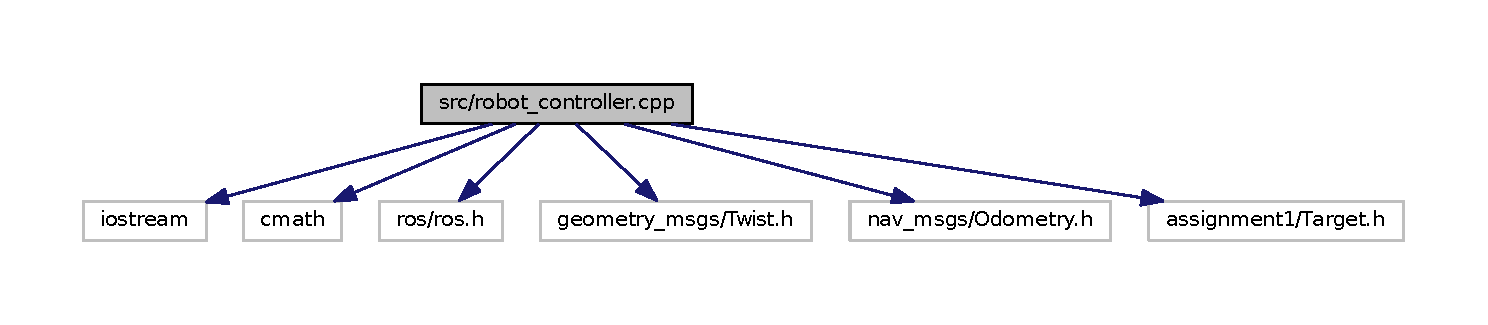
\includegraphics[width=350pt]{robot__controller_8cpp__incl}
\end{center}
\end{figure}
\subsection*{Functions}
\begin{DoxyCompactItemize}
\item 
void \hyperlink{robot__controller_8cpp_acaa43e6f70e8c71dadecf90fbaf7be9f}{position\+Callback} (const nav\+\_\+msgs\+::\+Odometry\+::\+Const\+Ptr \&pos)
\item 
int \hyperlink{robot__controller_8cpp_a3c04138a5bfe5d72780bb7e82a18e627}{main} (int argc, char $\ast$$\ast$argv)
\end{DoxyCompactItemize}
\subsection*{Variables}
\begin{DoxyCompactItemize}
\item 
ros\+::\+Publisher \hyperlink{robot__controller_8cpp_a65f3e154bdea4685affb99f01cc2f6ee}{pub\+\_\+speed}
\item 
ros\+::\+Subscriber \hyperlink{robot__controller_8cpp_a7487cfdd4aa66c85756101abadd5b3d4}{sub\+\_\+position}
\item 
nav\+\_\+msgs\+::\+Odometry \hyperlink{robot__controller_8cpp_a8a9990caf8ee110452f718bc2ee912d4}{target}
\item 
ros\+::\+Service\+Client \hyperlink{robot__controller_8cpp_a9615a83b719cce135f21ebd29a81e3bb}{target\+\_\+client}
\item 
assignment1\+::\+Target \hyperlink{robot__controller_8cpp_a18e31dc9dd6097bc7ce1628c0c38d770}{srv}
\item 
float \hyperlink{robot__controller_8cpp_a06f14a9abd47b91465f895d5259cdc1b}{distance} = 1000.\+0
\end{DoxyCompactItemize}


\subsection{Function Documentation}
\index{robot\+\_\+controller.\+cpp@{robot\+\_\+controller.\+cpp}!main@{main}}
\index{main@{main}!robot\+\_\+controller.\+cpp@{robot\+\_\+controller.\+cpp}}
\subsubsection[{\texorpdfstring{main(int argc, char $\ast$$\ast$argv)}{main(int argc, char **argv)}}]{\setlength{\rightskip}{0pt plus 5cm}int main (
\begin{DoxyParamCaption}
\item[{int}]{argc, }
\item[{char $\ast$$\ast$}]{argv}
\end{DoxyParamCaption}
)}\hypertarget{robot__controller_8cpp_a3c04138a5bfe5d72780bb7e82a18e627}{}\label{robot__controller_8cpp_a3c04138a5bfe5d72780bb7e82a18e627}
\index{robot\+\_\+controller.\+cpp@{robot\+\_\+controller.\+cpp}!position\+Callback@{position\+Callback}}
\index{position\+Callback@{position\+Callback}!robot\+\_\+controller.\+cpp@{robot\+\_\+controller.\+cpp}}
\subsubsection[{\texorpdfstring{position\+Callback(const nav\+\_\+msgs\+::\+Odometry\+::\+Const\+Ptr \&pos)}{positionCallback(const nav_msgs::Odometry::ConstPtr &pos)}}]{\setlength{\rightskip}{0pt plus 5cm}void position\+Callback (
\begin{DoxyParamCaption}
\item[{const nav\+\_\+msgs\+::\+Odometry\+::\+Const\+Ptr \&}]{pos}
\end{DoxyParamCaption}
)}\hypertarget{robot__controller_8cpp_acaa43e6f70e8c71dadecf90fbaf7be9f}{}\label{robot__controller_8cpp_acaa43e6f70e8c71dadecf90fbaf7be9f}


\subsection{Variable Documentation}
\index{robot\+\_\+controller.\+cpp@{robot\+\_\+controller.\+cpp}!distance@{distance}}
\index{distance@{distance}!robot\+\_\+controller.\+cpp@{robot\+\_\+controller.\+cpp}}
\subsubsection[{\texorpdfstring{distance}{distance}}]{\setlength{\rightskip}{0pt plus 5cm}float distance = 1000.\+0}\hypertarget{robot__controller_8cpp_a06f14a9abd47b91465f895d5259cdc1b}{}\label{robot__controller_8cpp_a06f14a9abd47b91465f895d5259cdc1b}
\index{robot\+\_\+controller.\+cpp@{robot\+\_\+controller.\+cpp}!pub\+\_\+speed@{pub\+\_\+speed}}
\index{pub\+\_\+speed@{pub\+\_\+speed}!robot\+\_\+controller.\+cpp@{robot\+\_\+controller.\+cpp}}
\subsubsection[{\texorpdfstring{pub\+\_\+speed}{pub_speed}}]{\setlength{\rightskip}{0pt plus 5cm}ros\+::\+Publisher pub\+\_\+speed}\hypertarget{robot__controller_8cpp_a65f3e154bdea4685affb99f01cc2f6ee}{}\label{robot__controller_8cpp_a65f3e154bdea4685affb99f01cc2f6ee}
\index{robot\+\_\+controller.\+cpp@{robot\+\_\+controller.\+cpp}!srv@{srv}}
\index{srv@{srv}!robot\+\_\+controller.\+cpp@{robot\+\_\+controller.\+cpp}}
\subsubsection[{\texorpdfstring{srv}{srv}}]{\setlength{\rightskip}{0pt plus 5cm}assignment1\+::\+Target srv}\hypertarget{robot__controller_8cpp_a18e31dc9dd6097bc7ce1628c0c38d770}{}\label{robot__controller_8cpp_a18e31dc9dd6097bc7ce1628c0c38d770}
\index{robot\+\_\+controller.\+cpp@{robot\+\_\+controller.\+cpp}!sub\+\_\+position@{sub\+\_\+position}}
\index{sub\+\_\+position@{sub\+\_\+position}!robot\+\_\+controller.\+cpp@{robot\+\_\+controller.\+cpp}}
\subsubsection[{\texorpdfstring{sub\+\_\+position}{sub_position}}]{\setlength{\rightskip}{0pt plus 5cm}ros\+::\+Subscriber sub\+\_\+position}\hypertarget{robot__controller_8cpp_a7487cfdd4aa66c85756101abadd5b3d4}{}\label{robot__controller_8cpp_a7487cfdd4aa66c85756101abadd5b3d4}
\index{robot\+\_\+controller.\+cpp@{robot\+\_\+controller.\+cpp}!target@{target}}
\index{target@{target}!robot\+\_\+controller.\+cpp@{robot\+\_\+controller.\+cpp}}
\subsubsection[{\texorpdfstring{target}{target}}]{\setlength{\rightskip}{0pt plus 5cm}nav\+\_\+msgs\+::\+Odometry target}\hypertarget{robot__controller_8cpp_a8a9990caf8ee110452f718bc2ee912d4}{}\label{robot__controller_8cpp_a8a9990caf8ee110452f718bc2ee912d4}
\index{robot\+\_\+controller.\+cpp@{robot\+\_\+controller.\+cpp}!target\+\_\+client@{target\+\_\+client}}
\index{target\+\_\+client@{target\+\_\+client}!robot\+\_\+controller.\+cpp@{robot\+\_\+controller.\+cpp}}
\subsubsection[{\texorpdfstring{target\+\_\+client}{target_client}}]{\setlength{\rightskip}{0pt plus 5cm}ros\+::\+Service\+Client target\+\_\+client}\hypertarget{robot__controller_8cpp_a9615a83b719cce135f21ebd29a81e3bb}{}\label{robot__controller_8cpp_a9615a83b719cce135f21ebd29a81e3bb}

\hypertarget{target__server_8cpp}{}\section{src/target\+\_\+server.cpp File Reference}
\label{target__server_8cpp}\index{src/target\+\_\+server.\+cpp@{src/target\+\_\+server.\+cpp}}
{\ttfamily \#include $<$iostream$>$}\\*
{\ttfamily \#include \char`\"{}ros/ros.\+h\char`\"{}}\\*
{\ttfamily \#include \char`\"{}geometry\+\_\+msgs/\+Twist.\+h\char`\"{}}\\*
{\ttfamily \#include \char`\"{}nav\+\_\+msgs/\+Odometry.\+h\char`\"{}}\\*
{\ttfamily \#include \char`\"{}assignment1/\+Target.\+h\char`\"{}}\\*
Include dependency graph for target\+\_\+server.\+cpp\+:\nopagebreak
\begin{figure}[H]
\begin{center}
\leavevmode
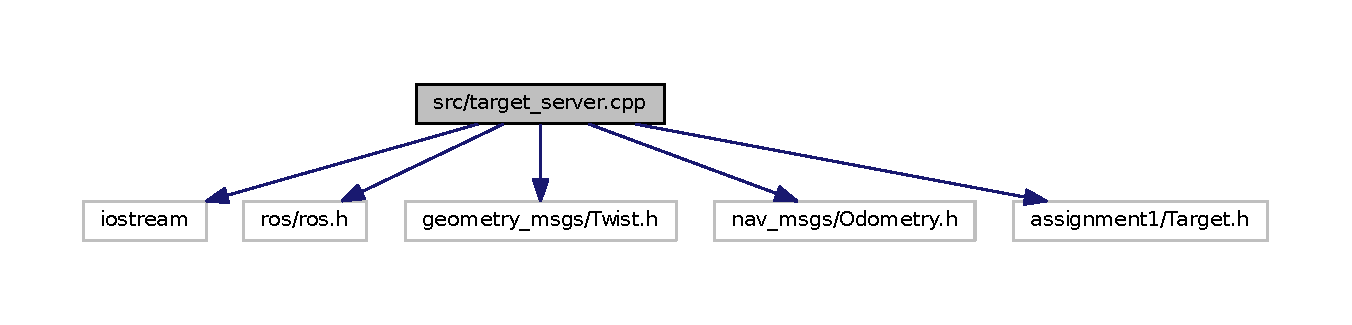
\includegraphics[width=350pt]{target__server_8cpp__incl}
\end{center}
\end{figure}
\subsection*{Functions}
\begin{DoxyCompactItemize}
\item 
float \hyperlink{target__server_8cpp_a8ada0dc1622d87a86740728e5f3656d7}{myrandom} (float minimum, float maximum)
\item 
bool \hyperlink{target__server_8cpp_a22312ae3149c8fb48ad9ade2c65277e7}{target\+Callback} (assignment1\+::\+Target\+::\+Request \&req, assignment1\+::\+Target\+::\+Response \&res)
\item 
int \hyperlink{target__server_8cpp_a3c04138a5bfe5d72780bb7e82a18e627}{main} (int argc, char $\ast$$\ast$argv)
\end{DoxyCompactItemize}


\subsection{Function Documentation}
\index{target\+\_\+server.\+cpp@{target\+\_\+server.\+cpp}!main@{main}}
\index{main@{main}!target\+\_\+server.\+cpp@{target\+\_\+server.\+cpp}}
\subsubsection[{\texorpdfstring{main(int argc, char $\ast$$\ast$argv)}{main(int argc, char **argv)}}]{\setlength{\rightskip}{0pt plus 5cm}int main (
\begin{DoxyParamCaption}
\item[{int}]{argc, }
\item[{char $\ast$$\ast$}]{argv}
\end{DoxyParamCaption}
)}\hypertarget{target__server_8cpp_a3c04138a5bfe5d72780bb7e82a18e627}{}\label{target__server_8cpp_a3c04138a5bfe5d72780bb7e82a18e627}
\index{target\+\_\+server.\+cpp@{target\+\_\+server.\+cpp}!myrandom@{myrandom}}
\index{myrandom@{myrandom}!target\+\_\+server.\+cpp@{target\+\_\+server.\+cpp}}
\subsubsection[{\texorpdfstring{myrandom(float minimum, float maximum)}{myrandom(float minimum, float maximum)}}]{\setlength{\rightskip}{0pt plus 5cm}float myrandom (
\begin{DoxyParamCaption}
\item[{float}]{minimum, }
\item[{float}]{maximum}
\end{DoxyParamCaption}
)}\hypertarget{target__server_8cpp_a8ada0dc1622d87a86740728e5f3656d7}{}\label{target__server_8cpp_a8ada0dc1622d87a86740728e5f3656d7}
\index{target\+\_\+server.\+cpp@{target\+\_\+server.\+cpp}!target\+Callback@{target\+Callback}}
\index{target\+Callback@{target\+Callback}!target\+\_\+server.\+cpp@{target\+\_\+server.\+cpp}}
\subsubsection[{\texorpdfstring{target\+Callback(assignment1\+::\+Target\+::\+Request \&req, assignment1\+::\+Target\+::\+Response \&res)}{targetCallback(assignment1::Target::Request &req, assignment1::Target::Response &res)}}]{\setlength{\rightskip}{0pt plus 5cm}bool target\+Callback (
\begin{DoxyParamCaption}
\item[{assignment1\+::\+Target\+::\+Request \&}]{req, }
\item[{assignment1\+::\+Target\+::\+Response \&}]{res}
\end{DoxyParamCaption}
)}\hypertarget{target__server_8cpp_a22312ae3149c8fb48ad9ade2c65277e7}{}\label{target__server_8cpp_a22312ae3149c8fb48ad9ade2c65277e7}

%--- End generated contents ---

% Index
\backmatter
\newpage
\phantomsection
\clearemptydoublepage
\addcontentsline{toc}{chapter}{Index}
\printindex

\end{document}
